% --------------------------------------------------
% Capítulo 5: AoM
% --------------------------------------------------
\chapter{Enhancing the Computation of Risk Zones Based on Emergency-Related Infrastructure in Smart Cities}\label{cap:aom}
\selectlanguage{english}

\begin{refsection}

\textbf{ABSTRACT}

In order to efficiently manage emergency situations in cities, it is crucial to have a well-distributed network of emergency response centres that can quickly initiate mitigation actions. Conversely, such infrastructure can also be leveraged when designing emergency management systems in smart cities. To enable this in any city, we have developed a risk classification system that uses open geospatial data to preprocess urban areas. For that, we exploited the previous concepts of Area of Interest (AoI) and Points of Interest (PoI), extending them to also incorporate the concept of Area of Mitigation (AoM) for any regular or irregular polygonal AoI, considerably enhancing the definition of risk perceptions in a city. Additionally, we have proposed a new algorithm that finds realistic positions for Event Detection Units (EDUs) based on the streets in a city, avoiding prohibited deployment areas, which was in fact a deficiency of previous algorithms for this problem. By potentially reducing the time required to detect and notify emergency events in more critical urban areas, we want to improve the performance of emergency management systems as a whole, bringing important contributions for smart city applications in this area.

\textbf{Keywords:} Urban emergency, Smart cities, Risk Zones, Risk maps, Emergency detection.

\section{Introduction}\label{sec:intro}

Urban areas are growing at an alarming rate, leading to a surge in emergency occurrences that require immediate action from first responders~\cite{Costa_2022}. From car accidents to building collapses, flooding, and fires, cities have faced a wide range of emergencies. In this scenario, hospitals, fire departments, police stations, and other response centres will play a critical role in mitigating the impact of such events~\cite{emergencies4,emergencies5}. Nevertheless, the effectiveness of these response centres depends on their strategic distribution across the city, which can significantly reduce the average response time. Researchers have then attempted to classify cities based on their risk of emergencies, but most of these efforts have focused on specific emergencies or regions. Hence, a more generalist approach that can be applied to any type of event and any region can be a valuable solution for planning effective emergency mitigation strategies in a smart city.

When an emergency occurs, every responder that can have a role in the related mitigation process should be notified and the proper actions to cease the causing event (or relieve its effects) will typically begin~\cite{Costa_2020,emergencies2}. Regardless of the type of emergency, first responders must move toward the affected area in order to take proper actions~\cite{emergencies3}. At this point, time is crucial, specially when critical events happen far from the available emergency response infrastructure. Therefore, any existing emergency detection system should be designed to leverage the already existing response centres in a city.

Leveraging open geospatial data about cities can offer valuable insights into the classification of urban areas and provide a clearer understanding of the challenges involved in initiating a mitigation action. Pre-processing urban geographic data to compute risk zones can help in planning different mitigation strategies based on varying risk perceptions~\cite{riskcities}. In fact, the risk perception of a city may differ depending on the parameters considered, but the ability to respond to an ongoing emergency will still be the ultimate goal~\cite{emergencies3}. By analysing open geospatial data, we can obtain a comprehensive view of the risk zones in a city and use this information to make informed decisions on emergency planning and management.

Our previous work in~\cite{riskzones} has defined the concepts of Area of Interest (AoI) and Points of Interest (PoI) regarding the classification of mitigation levels in a smart city. In that work, an initial perception of the risk level for each urban ``zone'' was proposed, taking as reference the distances of each zone to three different types of PoIs (hospitals, police stations, and fire departments). Actually, although the work in~\cite{riskzones} provided the initial mathematical fundamentals to compute risk perceptions based on the availability of mitigation facilities, the definition of the AoI and the practical exploitation of the computed maps could be inefficient and susceptible to errors. This way, an intuitive and flexible computational tool to support the definition of any AoI and the processing of computed zones would be valuable in many scenarios, specially when managing emergencies in smart city systems. Moreover, since such formulations would integrate different processing procedures considering geospatial data, with a modularized configuration that would allow future upgrades, the very definition of the AoI, PoI and mitigation zones (MZ) could be enhanced to extend the possibilities when dealing with urban risk zones.

The proper positioning of Event Detection Units (EDUs) is a critical decision that goes beyond the classification of an Area of Interest (AoI). Since such sensing units will be responsible for detecting events and notifying response centres, their positioning could be guided by the existence of PoIs within a city, particularly considering the definition of an AoI. In this sense, prioritising the positioning of EDUs in more risky zones - i.e., zones where it is more challenging to initiate an in-situ mitigation action - is essential to ensure timely detection and notification of events, reducing the response time in these areas. To this end, this work aims to enhance the classification of zones, including irregular AoIs (more flexible and realistic) and also Points of Interest (PoIs) outside the area of an AoI, since their influence can also be noticed. Additionally, we aim to improve the EDU positioning algorithm, which can serve as a planning tool for deploying sensing units in an AoI based on its risk levels. By improving the classification and placement of EDUs, we can enhance the effectiveness of emergency response efforts, potentially reducing the impact of emergencies on affected communities.

Therefore, the contributions of this paper can be highlighted as follows:

\begin{enumerate}
  \item The definition of an AoI as any regular or irregular polygon, instead of only rectangular areas as in~\cite{riskzones}, and the mathematical formulations for that;
  \item The adoption of Metro stations as an additional type of PoI, as well as the definition of the concept of Area of Mitigation (AoM);
  \item The proposal of a novel positioning algorithm that indicate EDUs positions respecting the risk factors of the zones and taking streets as the only feasible deployment areas;
  \item Experimental EDUs positioning results for the cities of Bucharest (Romania) and Porto (Portugal).
\end{enumerate}

The remainder of this paper is organised as follows. Section~\ref{sec:works} presents some related works. Section~\ref{sec:proposed_approach} presents the fundamental concepts of the proposed approach, while Section~\ref{sec:positioning} describes the new enhanced EDUs positioning algorithm. Experimental results are presented in Section~\ref{sec:simulation}, followed by conclusions and references.

%%%%%%%%%%%%%%%%%%
\section{Related works}\label{sec:works}

The problem of risk classification in smart cities has been studied by some researches that proposed approaches for tackling this issue in different ways. However, most of the works in the literature are specific for some cities or consider only a small set of emergencies types, lacking a generic approach that could be applied for any city regarding any emergency. As an example, the work in~\cite{Hung_2016} makes use of several input parameters to create a climate hazard resilience classification. Although it is enabled to work in any city, this approach is only suitable for climate hazards, missing other types of emergencies that may occur in an urban area.

Another example is the work in~\cite{Darabi_2019}. The authors proposed a flood risk maps modelling to prevent urban flood damage. They used rainfall data, land use, elevation and slope of terrain, curve number, distance to river, distance to channels, and depth of groundwater as input parameters. This is a good example of how several publicly available and unbiased data can be used to create a risk classification of regions in a city. But once again, that proposed approach was focused on flooding and other emergency types were not addressable by it, which might be an inherent limitation.

Many other works have presented approaches regarding specific emergencies as in~\cite{Hondula_2015,Maio_2018}, or specific cities as in\cite{Fernandez_2015}. Although some other works are more generic as the proposal in~\cite{Kontokosta_2018}, which makes use of several parameters to create a resilience index for smart cities, it requires the input of some locally-specific data. On the other hand, this work aims to create a framework that can make use of publicly available and unbiased data that are common for every city, creating a risk classification index that can be exploited in multiple ways.

Finally, we propose herein a comprehensive mathematical model to support mitigation level classification for smart cities, as well as a realistic EDUs positioning algorithm, relying only on publicly available and unbiased data and making it easier for implementation in any city. Moreover, our approach is not emergency-type specific, which is an advantage for large-scale implementations. Finally, since any type of PoI can be considered in the future, and the AoI and AoM concepts are highly configurable, we believe that smart city systems may acquire a practical tool by adopting our model, achieving combined contributions that were not addressed by previous works. 

%%%%%%%%%%%%%%%%%%%%%%%%%%%%
\section{Fundamentals of risk zones}\label{sec:proposed_approach}

% Area de Interesse
% - o que é
% - como é definida
% Zonas
% Polygonal AoI (acho que botar isso depois de PoIs, já que os assuntos se misturam)
% - mostrar a matemática para definir se uma zona tá dentro ou fora

To utilise our approach, an Area of Interest (AoI) must first be defined. The AoI is the region that will be classified by our mitigation level classification algorithm and have sensing units deployed. Thus, defining the AoI marks the beginning of the mitigation level classification process for a given region.

In~\cite{riskzones}, to classify a city region, a rectangular area that encompassed the city's entire perimeter had to be defined. Actually, the rectangular Area of Interest (AoI) might include zones outside the target region, which would affect the overall classification by including Points of Interest (PoI) that were not part of the region and influencing the computed risk levels of each zone during normalisation. Thus, if someone intended to classify the region of a city it was needed to define a rectangular area that comprised the perimeter of the whole city. Although it worked, some side effects were a concern, influencing the overall classification in two ways: a) including Points of Interest that were not part of the region and b) influencing the computed risk levels of each zone in the normalisation process.

In this sense, this work proposes a Polygonal AoI, changing the way an AoI is defined. Instead of a single rectangular area, the Polygonal AoI is a polygon of multiple edges contouring the region that needs to be classified, as shown in \figurename~\ref{fig:square_polygonal_aois}.

\begin{figure}[!ht]
  \centering
  \subfigure[Rectangular-shaped AoI for Porto.]{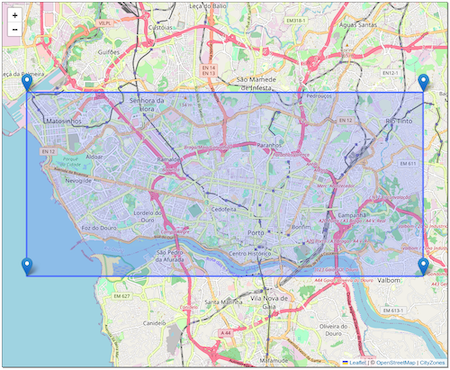
\includegraphics[width=0.7\linewidth]{Chapters/5-AoM/img/porto_square.png}}
  \hspace{0.5in}
  \subfigure[Polygonal AoI for Porto.]{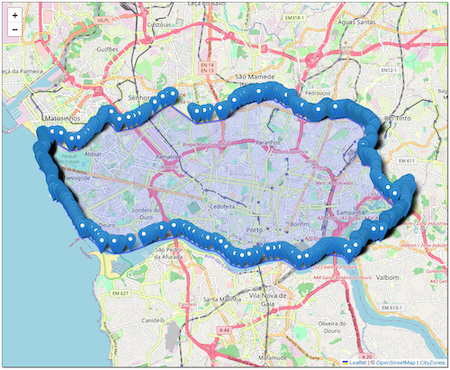
\includegraphics[width=0.7\linewidth]{Chapters/5-AoM/img/porto_polygon.png}}
  \caption{Comparison of rectangular-shaped and polygonal AoIs.}\label{fig:square_polygonal_aois}
\end{figure}

The figures show the differences when using a rectangular-shape AoI and a Polygonal AoI for the city of Porto. To classify the perimeter of the city of Porto, the best approach is to use a Polygonal Area of Interest. The rectangular-shaped AoI would include classification zones and Points of Interest outside the city's perimeter, which may not be of interest to a stakeholder.

Therefore, the use of a Polygonal AoI has the following advantages:

\begin{itemize}
  \item Focus on the region that will be classified and will have sensing units deployed;
  \item Do not let PoIs outside the region interfere the classification results;
  \item The mitigation levels of the zones are normalised against the whole AoI, thus, a Polygonal AoI avoids interference from other zones.
\end{itemize}

After the definition of the AoI, the whole area is divided in smaller squares of $zl$ meters length called zones. Each zone will get a risk perception $E$ that will produce the final classification. The $E$ is a value in the range $[0-1]$ that defines how far this zone is to response centres within the AoI. The value of $E$ of the zones are normalised, that is why having zones outside the AoI will interfere the final classification.

%%%%%%%%%
\subsection{Polygonal Areas of Interest}

% Modelar matematicamente o que é AoI

% Reaproveitar definição de Mitigation Zones

% Figure \ref{fig:check_zones_in_polygon} depicts the general idea when deciding if a zone is inside or outside the defined AoI, which is performed using geometry. 

The Polygonal AoI is a set of line segments $L$ defined by a set of points $P$ that can be connected to form a polygon surrounding the AoI. The set of points $P~=~\{P_0,~P_1,~...,~P_n\}$ is used to create the set of lines $L~=~\{P_0P_1,~P_1P_2,~...,~P_{n-1}P_n,~P_nP_0\}$. Only zones and PoIs inside the region delimited by the polygon are considered in the classification process of the AoI, i.e, PoIs outside the polygon are ignored and zones outside the AoI are not classified and also not inserted as input in the normalisation process.

Before starting the classification procedure it is needed to check which zones are inside the polygon defined by $L$. To do so, for each zone, our algorithm creates an imaginary line segment from the point defined by its localisation to the rightmost point possible (regarding the geolocalisation of the zones in our approach, in practical terms, it is a line segment from the coordinates of the zone to another coordinated located at the longitude 180º~E and at the same latitude). Next, the algorithm checks how many times the line segment crosses any line segment in $L$. If it crosses by an odd number of times, it is inside the polygon. \figurename~\ref{fig:check_zones_in_polygon} demonstrates this checking.

\begin{figure}[!ht]
  \centering
  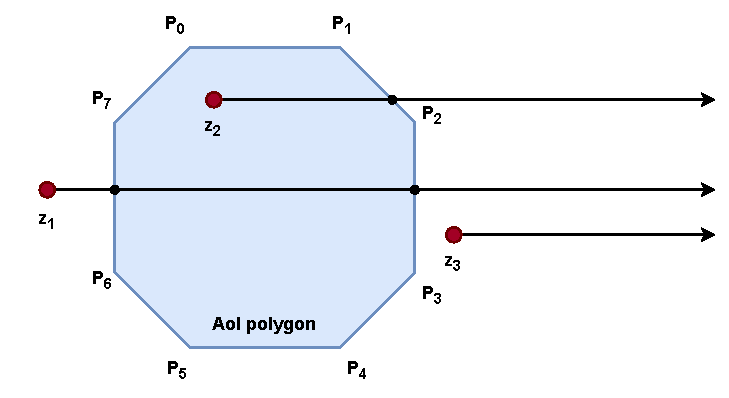
\includegraphics[width=0.7\linewidth]{Chapters/5-AoM/img/zones_inside_polygon.pdf}
  \caption{Checking if zones are inside an AoI polygon of any configuration. $z_2$ crosses the polygon line segments an odd number of times, so it is inside. The other zones are outside.}\label{fig:check_zones_in_polygon}
\end{figure}

In \figurename~\ref{fig:check_zones_in_polygon}, a Polygonal AoI formed by 8 points $P~=~\{P_0,~P_1,~P_2,~P_3,~P_4,~P_5,~P_6,~P_7\}$, making the polygon $L~=~\{P_0P_1,~P_1P_2,~P_2P_3,~P_3P_4,~P_4P_5,~P_6P_7,~P_7P_0\}$ is used as an example. In this scenario, three zones ($z_1$, $z_2$ and $z_3$) are checked against the polygon. The zones $z_1$ and $z_3$ cross the polygon line segments an even number of times (0 and 2, respectively), while the zone $z_2$ crosses the polygon line segments only once. This approach can be used to effectively check if a zone is inside the polygon, either regular or irregular. Thus, it is used to detect both zones and PoIs about being inside the Polygonal AoI before the classification process is started.

Although effective, this approach is very time consuming in Polygonal AoIs with too many points. Let $|Z|$ be the number of zones in the whole grid and $|P|$ the number of points that form the polygon, the time complexity of this algorithm is $O(|Z|\cdot|P|)$.

% FALAR ISSO NA SEÇÃO DE CITYZONES: Although the advantages described are significant, it is important to be aware that the computational cost of using a Polygonal AoI is higher because the classification algorithm has to check every zone in the map if it is inside the Polygonal AoI. This happens when using OpenStreetMap data as input to the algorithm because OpenStreetMap can export only rectangular areas of a region.

%%%%%%%%%
\subsection{Associating Points of Interest}\label{subsec:risk_zones}

% PoIs
% - o que são
% - como são definidos
% - falar sobre poder pegar PoIs fora das AoIs

By default, the classification approach only considers Points of Interest inside the Polygonal Area of Interest. While this is usually the desired behaviour for classification, there are scenarios where some PoIs are just outside the border of the Polygonal AoI. Excluding these PoIs may lead to incorrect classification of nearby zones. Although the AoI sets a hard limit on the zones to be classified, it may be useful to extend this limit and include certain PoIs in the classification process, making it a more realistic classification.% In a real emergency event, not only response centres within the area of the city will be requested. PoIs around the city's perimeter will also join the mitigation teams in such an event.

In this sense, our proposed approach makes use of an extension factor $I$ that will define how much the Polygonal AoI will be virtually extended, creating an Area of Mitigation (AoM) containing the PoIs that will be considered for classification of the AoI. This means that, although there will be a hard limit for zones, this limit will be extended for PoIs, i.e., PoIs that are out of the AoI by not more than the computed extended distance from the AoI will be included in the classification computation.

The computation of the extended distance $I_d$ is the multiplication of the extension factor $I$ by the average of the distances from the left-most to the right-most zone and the top-most and the bottom-most zone, as shown in Eq.~\ref{eq:extended_distance}. The depiction of the zones and the extended distance that creates the AoM are shown in \figurename~\ref{fig:extension_factor}.

\begin{equation}
  \label{eq:extended_distance}
  I_d = I \cdot \cfrac{dist(z_{top}, z_{bottom}) + dist(z_{left}, z_{right})}{2}
\end{equation}

\begin{figure}[!ht]
  \centering
  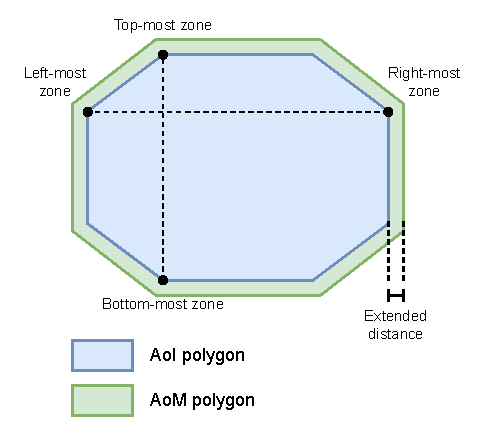
\includegraphics[width=0.7\linewidth]{Chapters/5-AoM/img/extension_factor.pdf}
  \caption{Computation of extended distance $I_d$ in a Polygonal AoI.}\label{fig:extension_factor}
\end{figure}

Once the extended distance is defined, the procedure for determining which Points of Interest to include in the classification process is similar to the method used for checking zones within the Polygonal Area of Interest. If a PoI does not meet the initial checking and is not inside the polygon, another verification is performed. The second checking calculates the distance of the PoI to the nearest zone in the Polygonal AoI. If this distance is less than or equal to the extended distance $I_d$, the PoI is inside the Area of Mitigation and will be included in the classification process.

\subsection{Computing the risk levels}

% Aqui é discutir o uso do log e porque o nosso é logn

In the classification of mitigation levels of the AoI, each zone will get a $ML$ that is the mitigation level class according to its distance to other PoIs within the AoI region. The goal of this classification method is to define how long it will take to initiate an \emph{in-loco} mitigation process in that zone. This way, zones that are far from response centres would take more time to have a response team at its location, in average. For that, the first step is to calculate the risk perception $E$ of each zone. The value $E$ is inversely proportional to the sum of the squared distance of the zone to every PoI within the AoI, as described in Equation~\ref{eq:risk_level_ch5}.

\begin{equation}
  \label{eq:risk_level_ch5}
  E(z_i) = \cfrac{1}{\displaystyle\sum_{j = 1}^{\lvert P \rvert}\left(\cfrac{1}{dist^2(z_i, p_j)} \cdot f(p_j)\right)} 
\end{equation}

The risk perception of a zone increases as it becomes more distant from the Points of Interest (PoIs). Once the risk perception of each zone is calculated, the mitigation level $ML$ is computed using the natural logarithm of the normalised value of its risk perception $E$, as shown in Equation~\ref{eq:risk_class_ch5}.

\begin{equation}
  \label{eq:risk_class_ch5}
  ML(z_i) = M - \min\left(M - 1, \left| \left\lceil \ln{\widehat{E}(z_i)} \right\rceil \right| \right)
\end{equation}

Our previous work in~\cite{riskzones} used a base 10 logarithm to compute the zone classification. However, we found that this approach produced confusing results in AoIs with several PoIs. In those cases, only a small area surrounding the PoIs would have $ML=1$ or even $ML=2$, while the majority of the AoI would be classified as $ML=3$ in a three-class configuration. Even though the classification of each zone is relative to the entire AoI, the base 10 logarithm created heatmaps that could mislead an observer into considering a region with many PoIs as a difficult-to-mitigate area due to the classification. As a result, we switched to using the natural logarithm in our current approach.

After several experimentation with other bases for the logarithm in the $ML$ formula, we found out that natural logarithm (base $\mathrm{e}$) works better for our scenarios, giving more meaningful heatmaps according to the position and presence of PoIs in an AoI. This is, in fact, a more common setting when processing different urban-related data since it provides more balanced representations~\cite{log1,log2}. 

After checking the zones inside the AoI, our algorithm then classifies the zones that were flagged \emph{inside} based on the position of the PoIs, allowing them to be considered for the defined Equations. This is a time consuming task because the algorithm has to calculate the mitigation level of each zone against every PoI. These tasks (checking zones inside the polygon and mitigation levels classification) should be performed in a multiprocessing approach for efficiency reasons. For example, the Python programming language provides a library for multiprocessing, enabling the program to make use of all cores and threads of the system CPU.\ Doing so, it is possible to create a pool of CPU workers and distribute groups of zones computations to them. %Each worker gets approximately the same number of zones to classify.

%%%%%%%
\section{Enhancing the positioning of the emergency detection units}\label{sec:positioning}

% Combining the local multiprocessing capability with the system architecture that allows for several workers to process tasks from the web application, CityZones has two layers of multiprocessing at all.

After the classification process, it is possible to position the EDUs according to the risk level of each zone. The work in~\cite{riskzones} presented an initial Random algorithm that only demonstrated how the concept of risk zones could be leveraged to position EDUs in a city. In fact, that algorithm makes no consideration about prohibited deployment areas, making it unrealistic in real scenarios. 

In~\cite{sustainable}, we proposed different algorithms for EDUs positioning following our concept of risk zones based on existing emergency mitigation infrastructure. Among the proposals, the Restricted EDU algorithm stands out as a positioning approach that rely on an initial uniform distribution, but that also perform further adjustments to position EDUs only on allowed zones (streets). However, although the results were promising, the Restricted algorithm may result in a poorly distributed set of units in some cases. The envisioned flaws in that algorithm fostered the development of an improved version, described in this section. 

Let's take as an example an AoI comprising a heterogeneous region (streets, land and ocean) like the one presented in \figurename~\ref{fig:porto_oceano_restricted}. In that Figure, three different risk classes were considered and the AoI was classified accordingly, showing the suggested positions by the Restricted algorithm in~\cite{sustainable}. 

\begin{figure}[!ht]
  \centering
  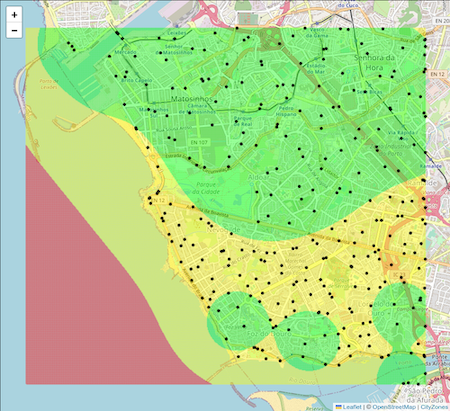
\includegraphics[width=0.7\linewidth]{Chapters/5-AoM/img/porto_oceano_restricted.png}
  \caption{A square AoI over the city of Porto, covering both urban and beach areas. EDUs are positioned by the Restricted algorithm.}    \label{fig:porto_oceano_restricted}
\end{figure}

We propose now the Enhanced algorithm, which follows a different positioning approach. This algorithm computes how distant an EDU must be to another in order to get an uniform distribution considering a small region around roads and streets. In our experiments, we are using a 100~m space around the permitted zones as coverage area for this computation, as shown in \figurename~\ref{fig:restricted_plus_area}, but other configuration could be adopted. Since our basic assumption is that the EDUs positioning is not allowed to be outside roads and streets, it does not make sense to consider the whole AoI area to be covered, making the proposed solution more adequate for smart city scenarios.

\begin{figure}[!ht]
  \centering
  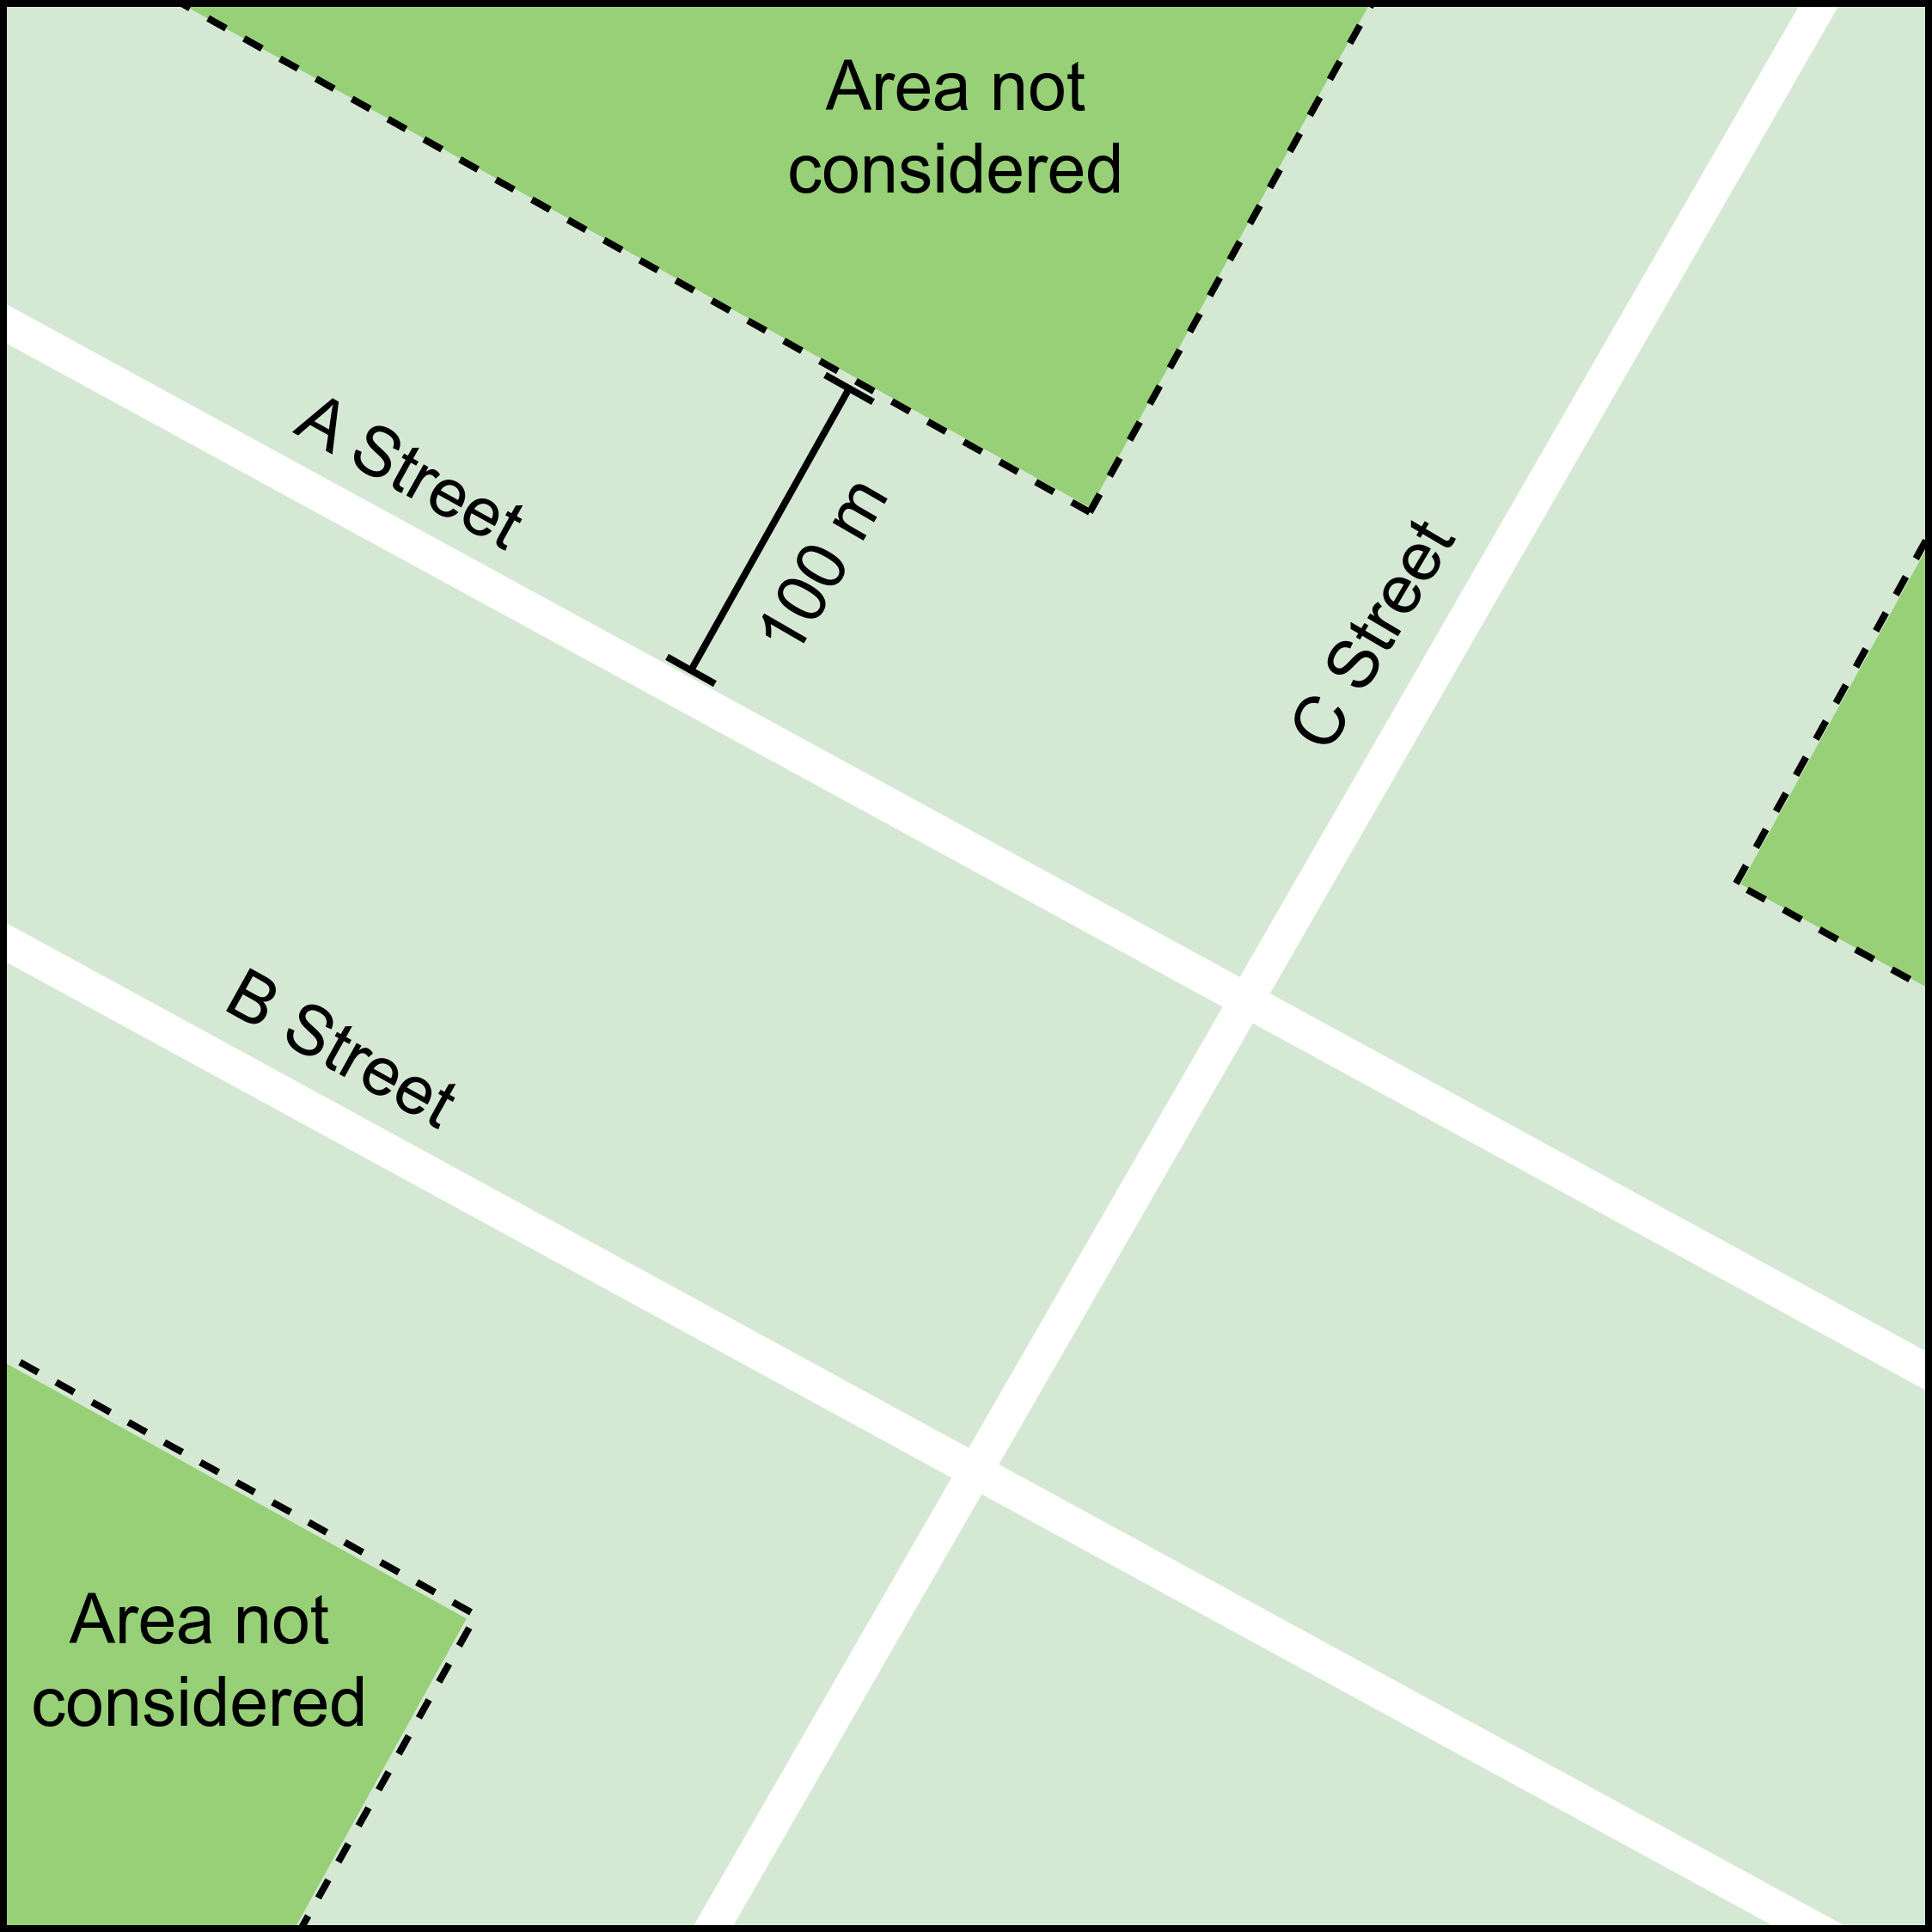
\includegraphics[width=0.7\linewidth]{Chapters/5-AoM/img/restricted_plus_area.png}
  \caption{A schematic representation for the operation of the Enhanced EDUs positioning algorithm.}\label{fig:restricted_plus_area}
\end{figure}

After computing the minimum distance between EDUs, the Enhanced algorithm visits the permitted zones inside the AoI and verifies if it is possible to deploy an EDU in that zone. The possibility to deploy is true if the zone is far enough from another EDU, i.e, there are no EDUs in the surroundings that breaks the minimum distance restriction computed in the previous step. By doing this, the Enhanced algorithm is capable of deploying emergency detection units uniformly across the permitted zones inside an AoI. \figurename~\ref{fig:porto_oceano_restricted_plus} demonstrate the distribution of EDUs using the Enhanced algorithm in the same scenario that the Restricted algorithm made a poor distribution.

\begin{figure}[!ht]
  \centering
  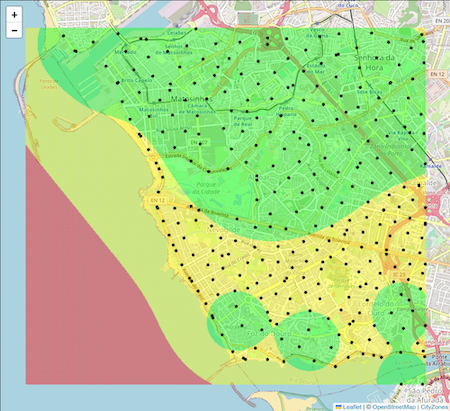
\includegraphics[width=0.7\linewidth]{Chapters/5-AoM/img/porto_oceano_restricted_plus.png}
  \caption{A square AoI over the city of Porto, covering both urban and beach areas. EDUs are positioned by the Enhanced algorithm.}\label{fig:porto_oceano_restricted_plus}
\end{figure}

As shown in \figurename~\ref{fig:porto_oceano_restricted_plus}, the EDUs are more evenly distributed in such a heterogeneous scenario if using the Enhanced algorithm, which we believe may be more valuable for different configurations of AoI, both square-shaped and following polygonal configurations. This new distribution can make a better use of the limited number of EDUs that are available for deployment, avoiding unnecessary overlapping.

%All the algorithms but Random need that the position of the former EDU is already defined to calculate the position of the next. Because of that, it is not possible to make use of the multiprocessing capabilities in this task.

%After classification and positioning, the RiskZones tool save the resulting data in CSV files. Those files are used by the worker application to send back the results to the web application.

%%%%%%%%%%%%%%
\section{Simulations results}\label{sec:simulation}

%To implement the proposed approach for classification and EDUs positioning, we developed a web application called CityZones. Its development has began with the work in \color{red}[?? SoftwareX]\color{black}, implementing the first version of the classification algorithms and the Random, Balanced, Balanced+ and Restricted positioning algorithms. The current version implements the Polygonal AoI, the extension factor for AoM and the Restricted+ positioning algorithm. The tool is publicly available at \emph{https://cityzones.just.pro.br} and can be used after the registration procedure.

To implement the proposed approach for risk zones classification, as well as EDUs positioning based on the Enhanced algorithm, we implemented their functions in the Python programming language with support of multiprocessing and geojson libraries. The polygonal definition of the AoI was allowed with the manual definition of the points to be considered, which are inserted into an input text file and that can be retrieved from open databases. The computed results are displayed as maps to be exhibited by a web browser.

As a demonstration of the proposed enhancements in this paper, we used a GeoJSON file for the boundaries of the city of Bucharest, Romania, which were used to define the Area of Interest for the simulations. The Polygonal AoI used for this simulation was composed of 356~points, had a zone length of 10~m, selecting a total of 2,407,778~zones inside the defined polygon. The extension factor for the creation of the AoM was of $I~=~10\%$, collecting a total of 156~PoIs for the classification process. Both the Restricted and the new Enhanced algorithms were tested in this scenario with a value of $U~=~300$ (available number of EDUs for positioning). The purpose of this simulation is to experiment the new proposals described in this paper and how well the Enhanced algorithm performs in a regular city scenario.

\figurename~\ref{fig:bucharest_restricted} shows the results of the classification and how the EDUs were positioned within the Polygonal AoI of Bucharest. The EDUs were positioned prioritising the more risky zones -- marked as red --, i.e, zones in which a \emph{in-loco} mitigation would take longer because of their distance from response centres (PoIs) compared to other zones in the same AoI. Although the Restricted algorithm worked as expected, deploying sensing units only in permitted zones (in this case, streets and roads), its distribution was not very homogeneous. It is noticeable that in some regions there are two or more EDUs too close while there are other regions with EDUs too far from each other, reducing their actual coverage. This misplacing of EDUs causes unnecessary overlapping as also uncovered zones in the AoI. This fact happened even with the existence of some permitted zones that could allow a better positioning configuration.

\begin{figure}[!ht]
  \centering
  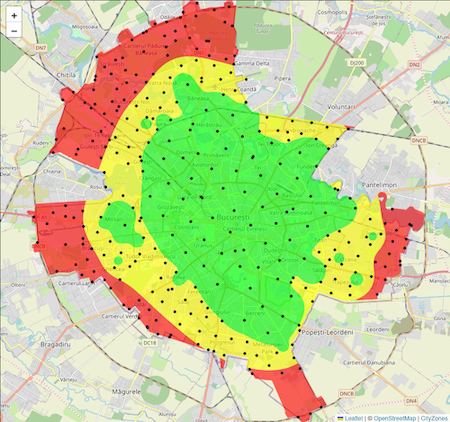
\includegraphics[width=0.7\linewidth]{Chapters/5-AoM/img/bucaresti_restricted.png}
  \caption{Results for the Restricted positioning algorithm in Bucharest.}\label{fig:bucharest_restricted}
\end{figure}

The second simulation considered the Enhanced positioning algorithm, with the results being shown in \figurename~\ref{fig:bucharest_restricted_plus}. In this result, it is clearer that the new positions for the EDUs make a more uniform distribution, considering the permitted zones. The same regions that got too many or too few sensing units in the Restricted algorithm now are more regular, even with the restriction of using only streets and roads as allowed deployment areas. Such uniformity could eventually result in a better distribution concerning network coverage and emergencies detection, but such type of quality evaluation was left to future works. 

\begin{figure}[!ht]
  \centering
  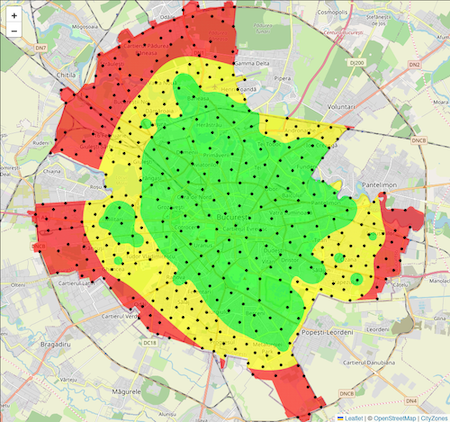
\includegraphics[width=0.7\linewidth]{Chapters/5-AoM/img/bucaresti_restricted_plus.png}
  \caption{Results for the Enhanced positioning algorithm in Bucharest.}\label{fig:bucharest_restricted_plus}
\end{figure}

Finally, the Enhanced algorithm performed faster than the compared Restricted algorithms. For the same Polygonal AoI, the Restricted algorithm took 170.253~seconds while the Enhanced algorithm took only 55.748~seconds, a reduction of 67.25\% of processing time. All tasks were performed on an AMD~Ryzen~5~4600H~3.0~GHz~CPU running in a computer with 16~GiB~RAM.\

\section{Conclusions}\label{sec:conclusion}

This paper presented the enhancements for the classification and EDUs positioning approaches for emergencies management in smart cities, significantly improving our previous results. First, such new enhancements were centred on the definition of Polygonal AoI, making it possible to define AoIs of irregular forms instead of following a limiting rectangular-shaped area. Second, the concept of Area of Mitigation (AoM) was introduced, which is an important extension of the AoI to include any number of PoIs in the surroundings of the AoI, avoiding the use of the AoI's perimeter as a hard limit for PoIs inclusion. Third, an improved computation of the risk level was defined, achieving a more robust formulation. Finally, a new EDUs positioning algorithm was proposed, which performs a restrictive streets-based distribution but achieving a more uniform EDUs positioning configuration that might have a better impact on emergencies detection as a whole. 

The proposed enhancements were validated through simulations considering real data, taking as reference the city of Bucharest, Romania. In our simulations, the Polygonal AoI was of great importance, since Bucharest's borders has an irregular shape, making it possible to limit the classification of zones inside the city's perimeter. In the defined AoI, the Enhanced algorithm performed better than the Restricted, placing the sensing units in a more uniform manner and also improving the coverage area of the EDUs. Finally, regarding the computational cost of the algorithms, the Enhanced performed 67.25\% faster, making it more suitable when computing a large quantity of sensors in a large area. 

Future works will perform additional simulations in other cities, further assessing the performance of the Enhanced algorithm. Moreover, additional computation metrics will be defined to better support comparisons among different positioning algorithms.

\printbibliography[heading=subbibliography]
\end{refsection}
% \selectlanguage{brazil}
